\documentclass[12pt]{ctexart}
\usepackage{amsmath}
\usepackage{wasysym}
\usepackage{graphicx}
\usepackage{caption}
\usepackage{subfigure}
\title{\textbf{NOIP模拟赛2}}
\author{GGN\&HJQ}
\date{2020年8月16日18:00-21:00}
\begin{document}
	\maketitle
	\begin{center}
		\begin{tabular}{|c|c|c|c|}
			\hline 题目名称&多米诺骨牌&抽卡&归程\\
			\hline 英文名称&domino&card&return\\
			\hline 源文件名&domino.cpp&card.cpp&return.cpp\\
			\hline 输入文件名&domino.in&card.in&return.in\\
			\hline 输出文件名&domino.out&card.out&return.out\\
			\hline 题目类型&传统&传统&传统\\
			\hline 时间限制&1s&1s&1s\\
			\hline 空间限制&512MB&512MB&512MB\\
			\hline 测试点数目&10&10&10\\
			\hline 每个测试点分值&10&10&10\\
			\hline
		\end{tabular}
	\end{center}
	\textbf{注意事项}\\
	1.评测环境:ubuntu18.04 lts 64位,CPU为Intel Core i7-8550U\\
	2.评测软件:lemon\\
	3.编译工具:g++10.1.0\\
	3.编译命令:g++ -o \%s \%s.cpp -lm (\%s为题目英文名)\\
	4.比较方式:全文比较,忽略行末空格和文末回车\\
	5.请不要直接从题面中复制样例\\
	6.比赛时可以向cppascalinux提交源程序进行评测,但是只返回编译信息,且最终评测结果以最后一次提交为准\\
	7.$AK$的选手会收到神秘大礼qwq
	\newpage
	\section{多米诺骨牌}
	\subsection{题目背景}
	HJQwQ在玩多米诺骨牌,但他已经玩腻了摆放然后推倒的玩法.于是他找来了国际象棋棋盘,开始往上面摆骨牌.这时他突发奇想:棋盘上最多能摆多少个不相邻的骨牌?但是他还要去打MC,于是把这个问题留给了你
	\subsection{题目描述}
	有一个$n$行$m$列($n\times m$)的棋盘,在它的上面放若干张$1\times2$或$2\times1$的骨牌,要求骨牌必须完全位于棋盘内,每个格子至多只被一张骨牌覆盖,且这些骨牌两两不相邻(我们定义两张骨牌是"相邻"的,当且仅当这两个骨牌至少有一条公共边或一个公共顶点,如图1和图2中的两个骨牌是相邻的,而图3中的两个骨牌不相邻),求最多可以摆放骨牌的数目

	\begin{figure}[htbp]
		\centering
		\begin{minipage}[t]{0.3\textwidth}
			\centering
			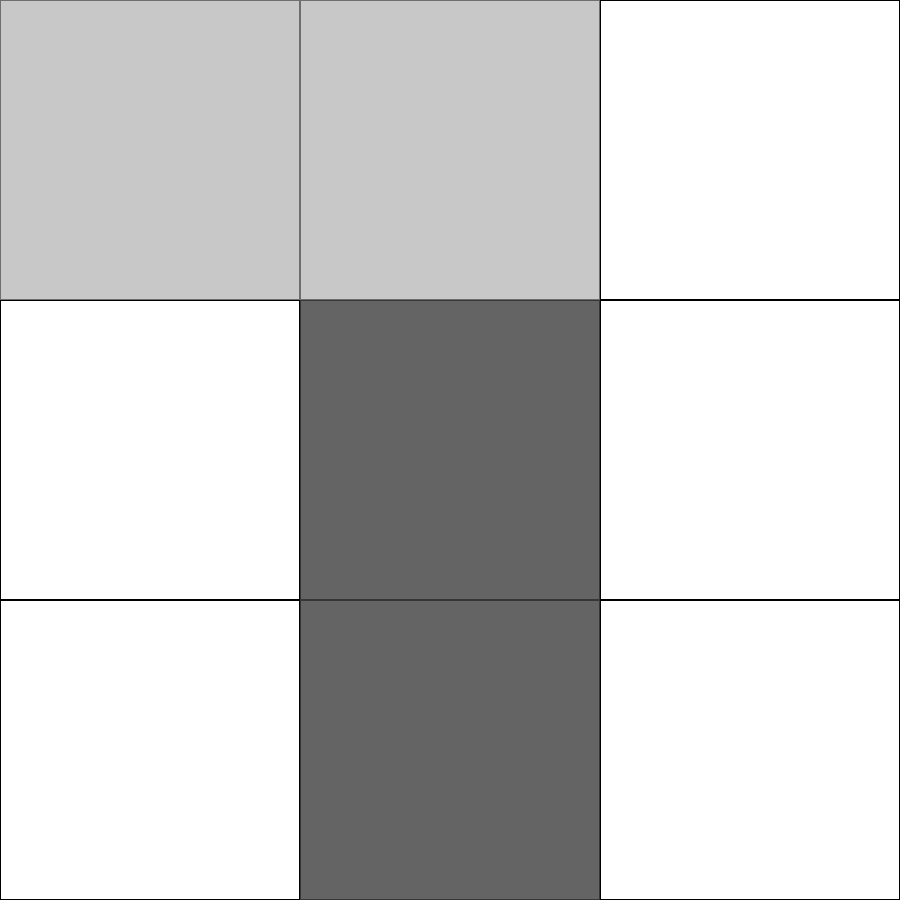
\includegraphics{pictures/1-1.png}
			\caption{}
		\end{minipage}
		\begin{minipage}[t]{0.3\textwidth}
			\centering
			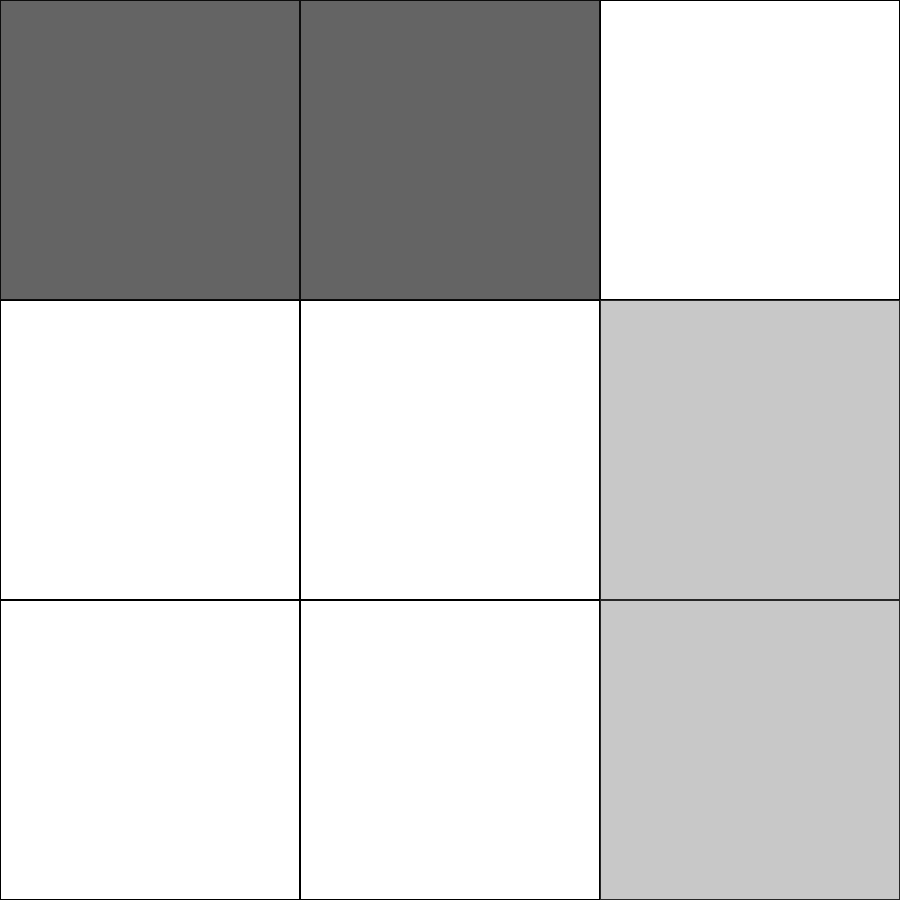
\includegraphics{pictures/1-2.png}
			\caption{}
		\end{minipage}
		\begin{minipage}[t]{0.3\textwidth}
			\centering
			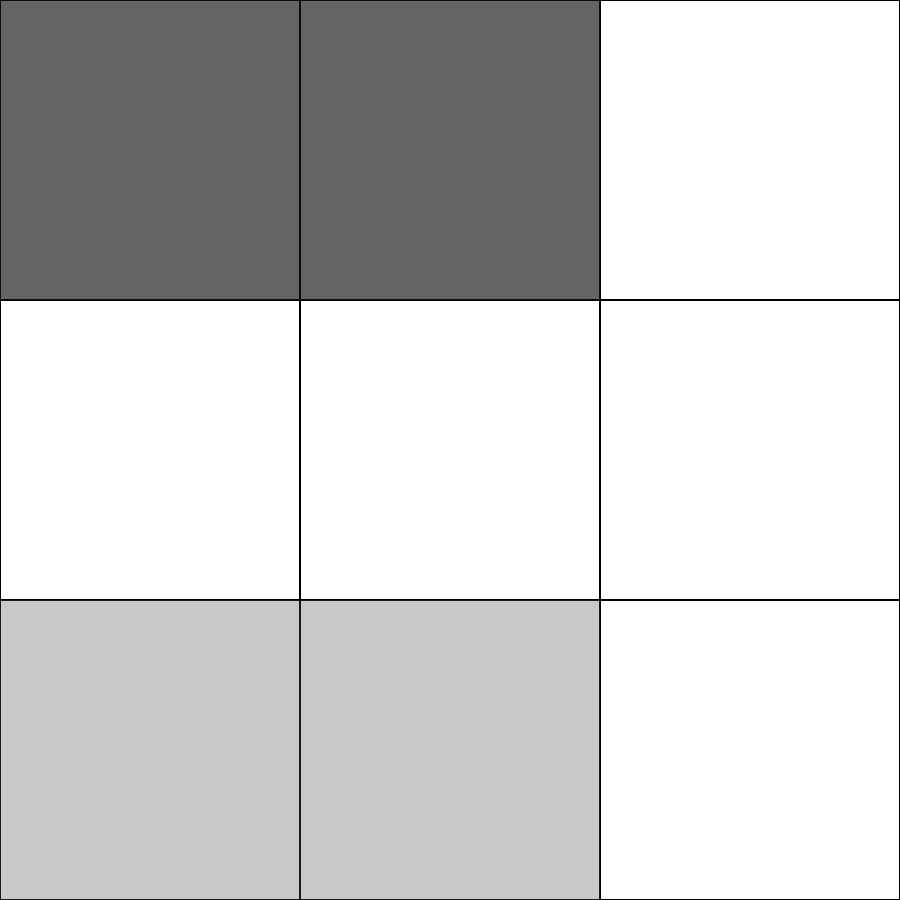
\includegraphics{pictures/1-3.png}
			\caption{}
		\end{minipage}
	\end{figure}

	\subsection{输入格式}
	第一行一个正整数$T$,表示数据组数
	接下来$T$行,每行两个正整数$n,m$
	\subsection{输出格式}
	共$T$行,每行一个正整数,表示对于每组数据的答案
	\subsection{输入输出样例}
	\begin{center}
		\begin{tabular}{|p{6cm}|p{6cm}|}
			\hline domino.in&domino.out\\
			\hline	5&1\\
					1 2&2\\
					3 2&6\\
					5 5&5\\
					4 6&9\\
					5 8&\\
			\hline
		\end{tabular}
	\end{center}
	\subsection{样例解释}
	对于5组数据,各给出一种可行的方案(图4$\to$图8),不难证明都是最大方案

	\begin{figure}[htbp]
		\centering
		\begin{minipage}[t]{0.32\textwidth}
			\centering
			
\includegraphics[width=0.5\textwidth]{pictures/2-1.png}
			\caption{}
		\end{minipage}
		\begin{minipage}[t]{0.32\textwidth}
			\centering
			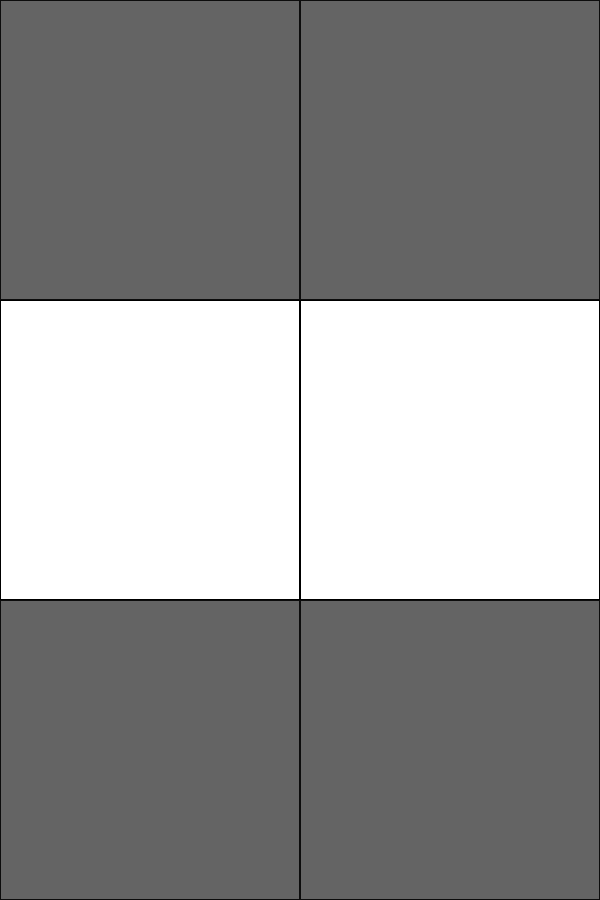
\includegraphics[width=0.5\textwidth]{pictures/2-2.png}
			\caption{}
		\end{minipage}
		\begin{minipage}[t]{0.32\textwidth}
			\centering
			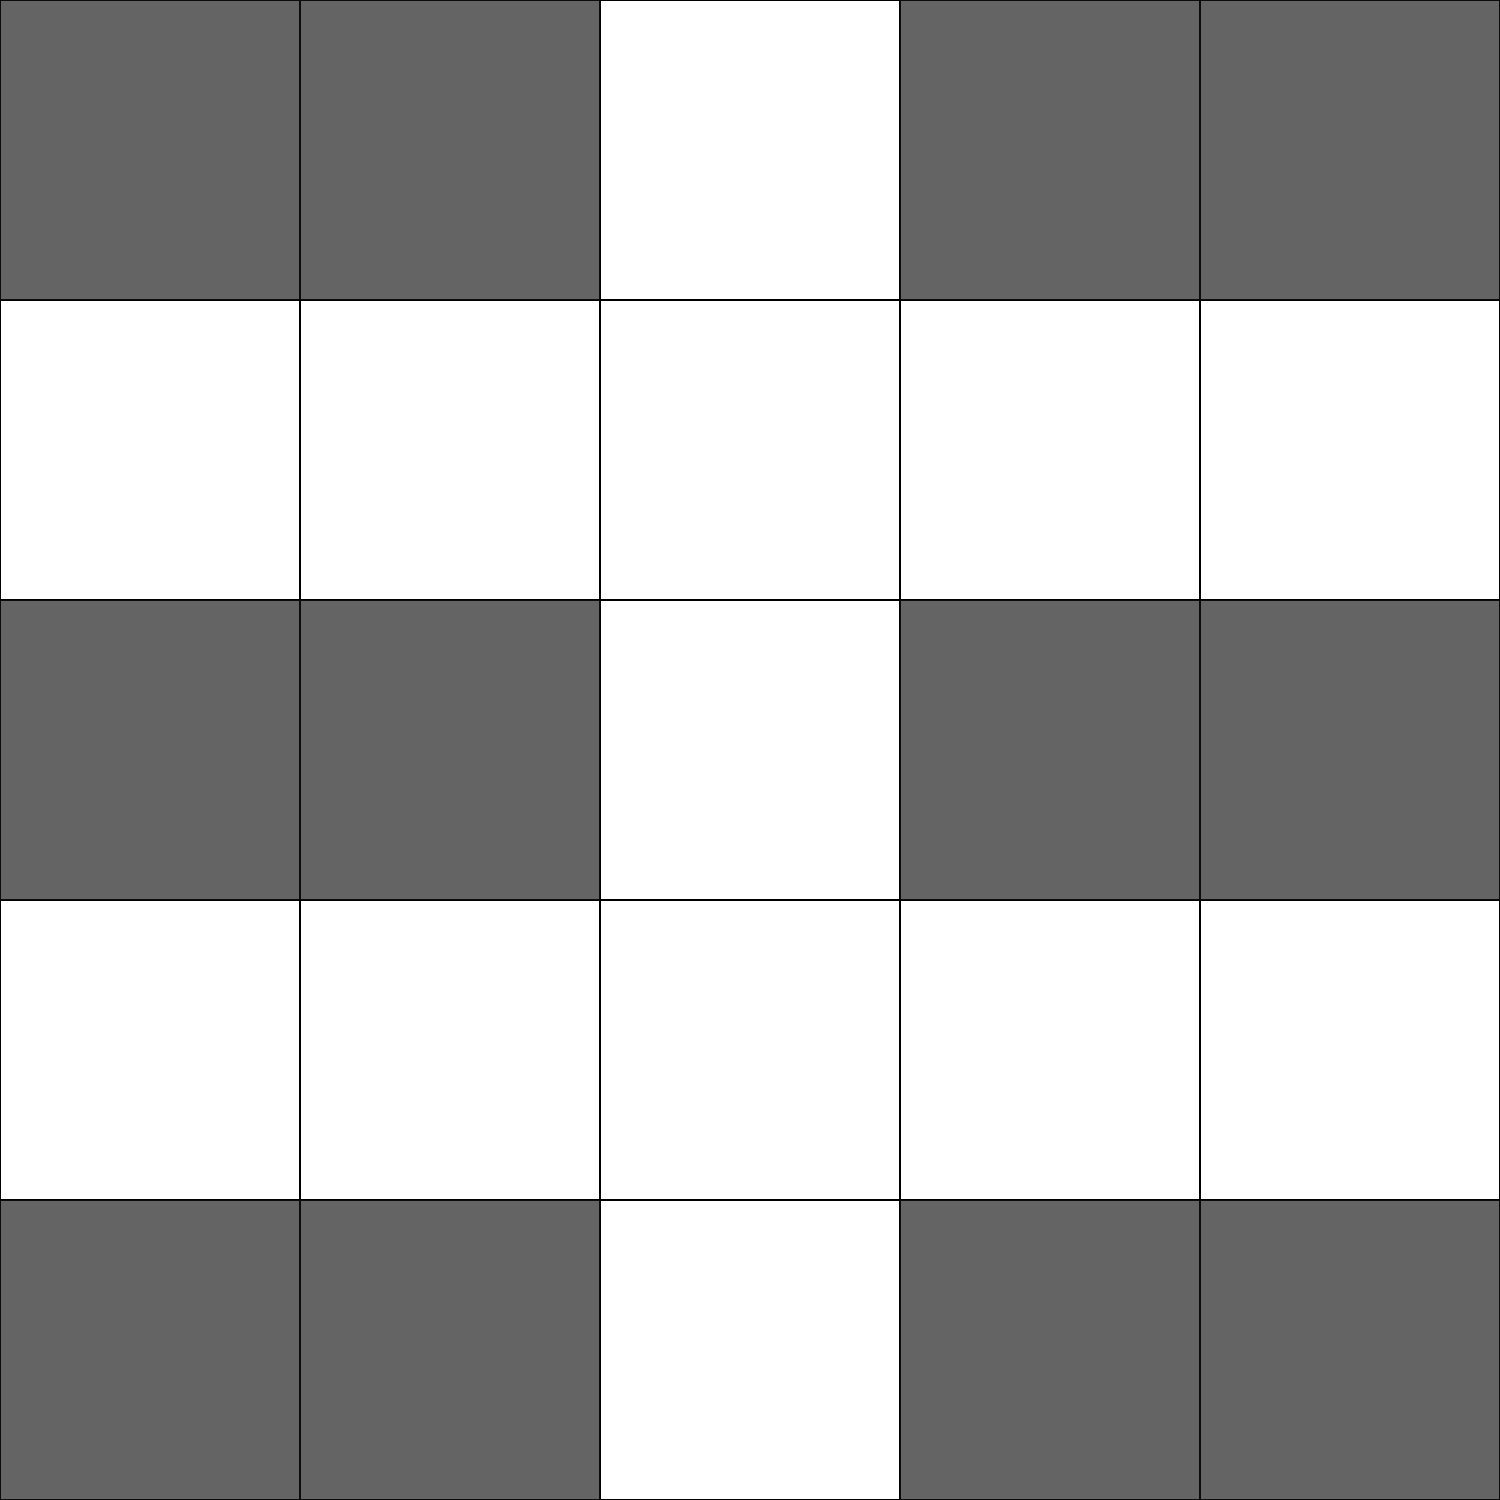
\includegraphics[width=\textwidth]{pictures/2-3.png}
			\caption{}
		\end{minipage}
	\end{figure}

	\begin{figure}[htbp]
		\centering
		\begin{minipage}[t]{0.49\textwidth}
			\centering
			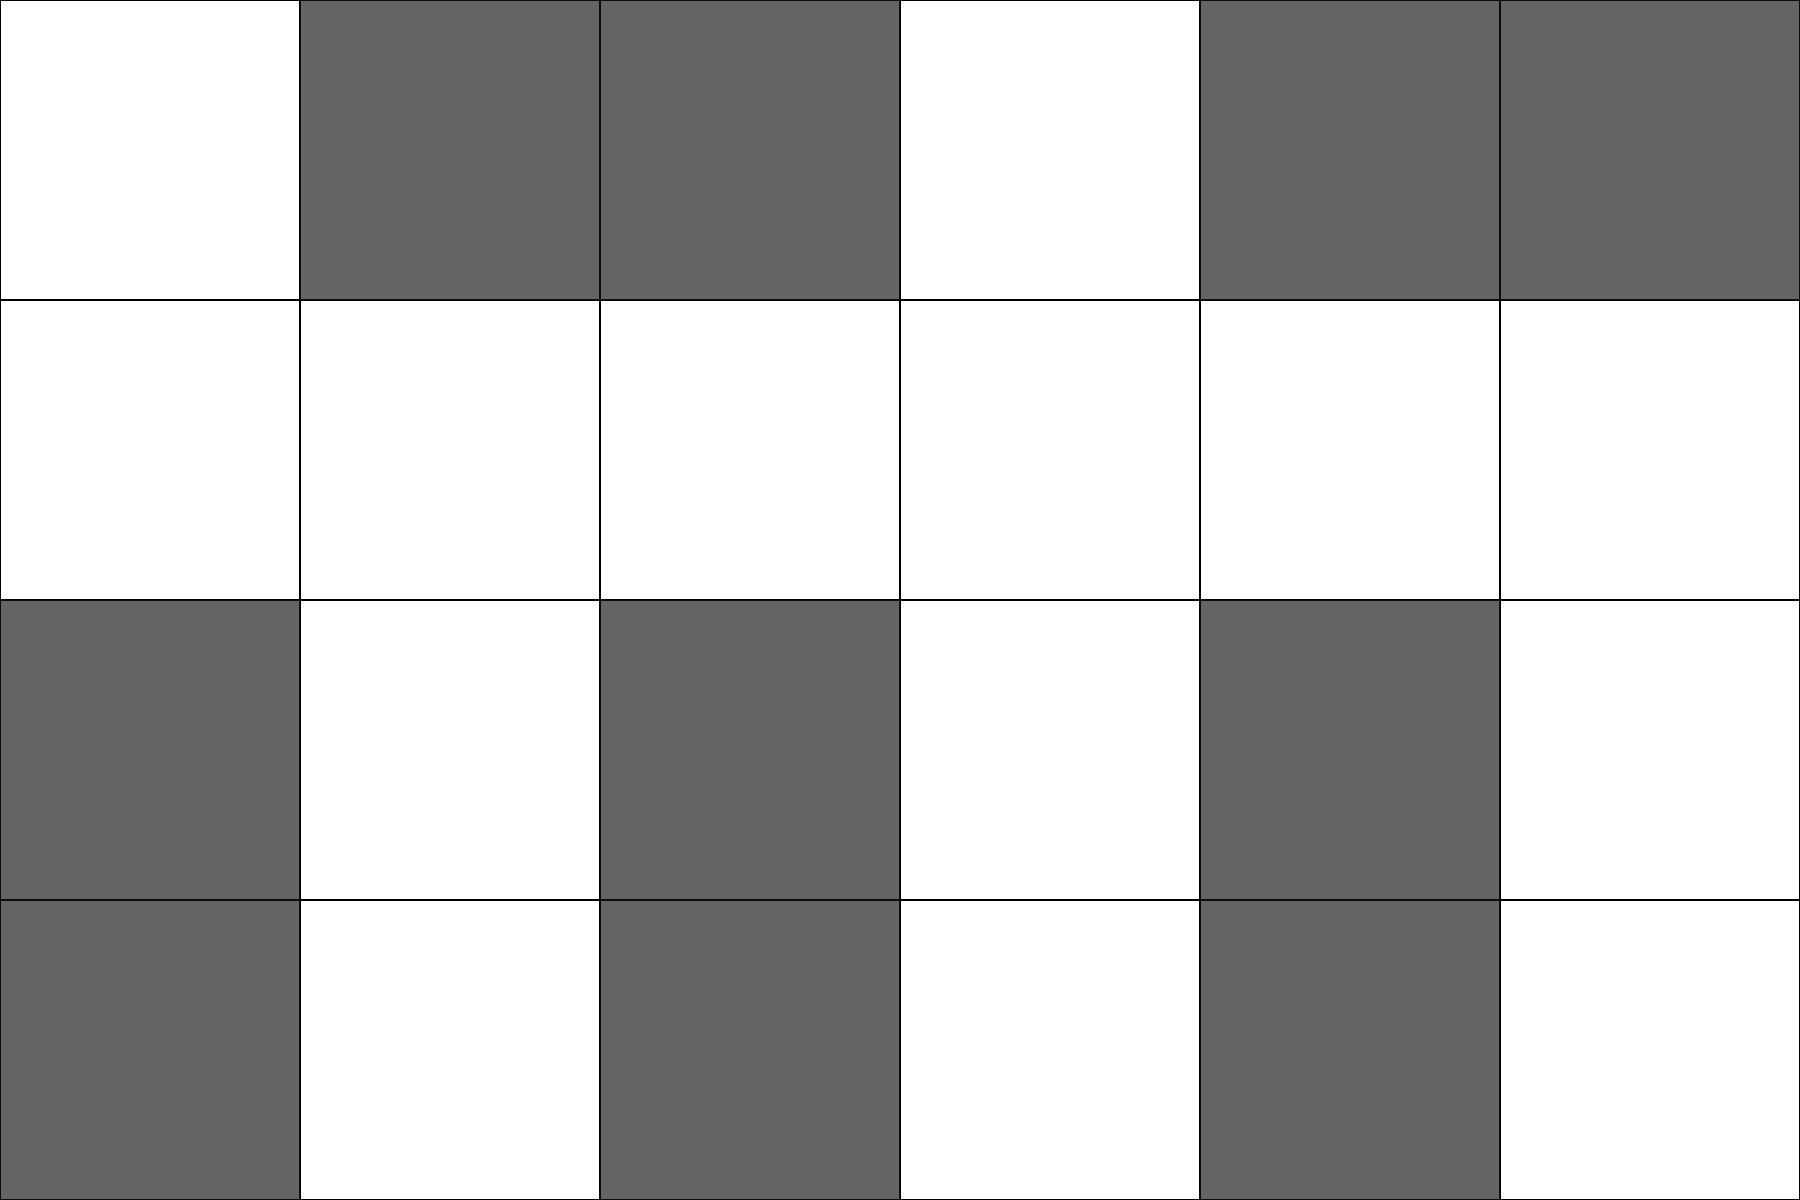
\includegraphics[width=0.8\textwidth]{pictures/2-4.png}
			\caption{}
		\end{minipage}
		\begin{minipage}[t]{0.49\textwidth}
			\centering
			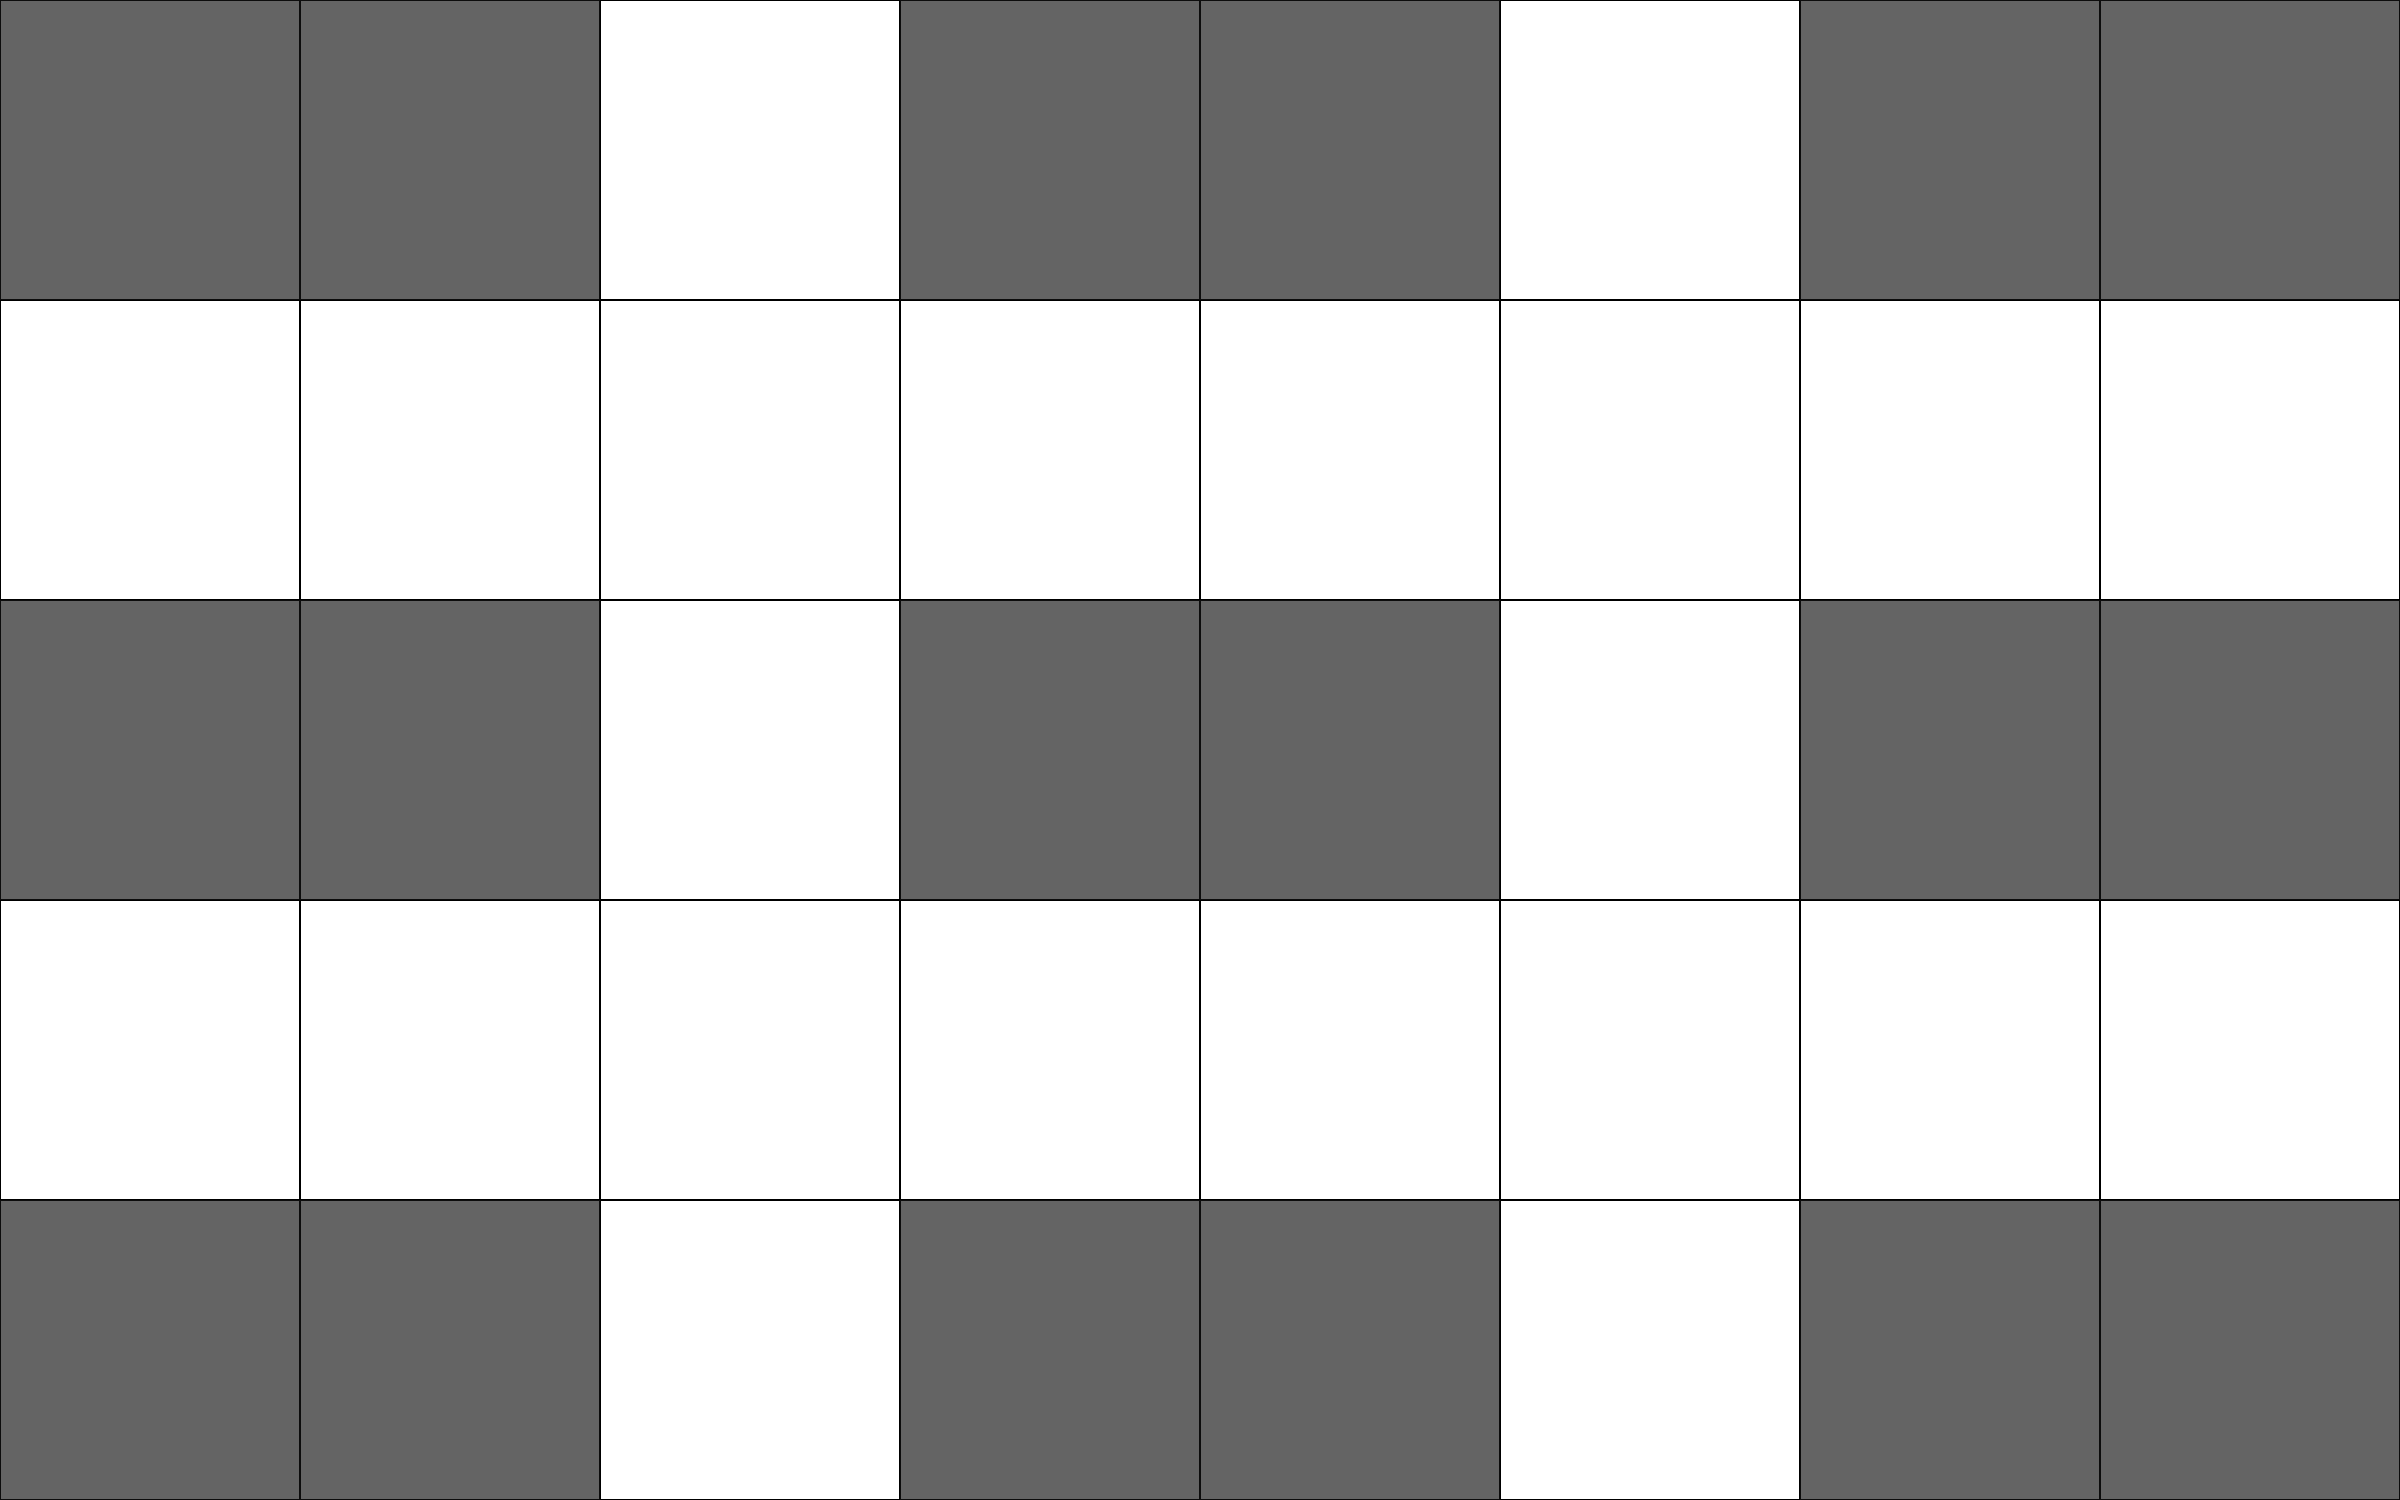
\includegraphics[width=\textwidth]{pictures/2-5.png}
			\caption{}
		\end{minipage}
	\end{figure}

	\subsection{数据范围}
	\begin{center}
		\begin{tabular}{|c|c|c|}
			\hline 测试点编号&$n$&$m$\\
			\hline 1&$=1$&$\le10$\\
			\hline 2,3&$\le2$&$\le10^5$\\
			\hline 4,5&$\le5$&$\le10^5$\\
			\hline 6,7&$\le10$&$\le1000$\\
			\hline 8,9,10&$\le10^5$&$\le10^5$\\
			\hline
		\end{tabular}
	\end{center}
	对于100\%的数据,有$1\le T\le10,1\le n,m\le10^5$
	\newpage
	\section{抽卡}
	\subsection{题目背景}
	HJQwQ在和GGN玩一个抽卡游戏.他们的面前摆放着$n$张背面朝上的卡,每张卡的正面印着一个价值$v_i$. HJQwQ可以从中抽走$k$张,并获得这些卡上所有的价值.擅长出老千的HJQwQ早就看穿了每张卡的价值,然而机智的GGN更早就料到HJQwQ会出老千,于是他又加了一条规则:取出的k张卡的位置必须两两不相邻.这下HJQwQ方了:他该抽走哪些卡,才能使的自己获得的总价值最大?
	\subsection{题目描述}
	有一个长为$n$的数组$v_i$,请从中选出$k$个不相邻的位置,使得这些位置的和最大,并输出这个和,你需要对$k\in\left[1,\lfloor\frac{n+1}2\rfloor\right]$都输出一个答案
	\subsection{输入格式}
	第一行一个正整数$n$

	第二行$n$个用空格分隔的正整数$v_1\sim v_n$
	\subsection{输出格式}
	共$\lfloor\frac{n+1}2\rfloor$行,每行一个正整数,第$i$行的正整数表示$k=i$时的答案
	\subsection{输入输出样例}
	\subsubsection{样例1}
	\begin{center}
		\begin{tabular}{|p{6cm}|p{6cm}|}
			\hline card.in&card.out\\
			\hline	10&9\\
					7 3 2 7 2 7 4 9 9 1&16\\
					&23\\
					&30\\
					&31\\
			\hline
		\end{tabular}
	\end{center}
	见下发文件中的card1.in/card1.out
	\subsubsection{样例解释}
	$k=1$时,抽$v_8=9$最大

	$k=2$时,抽$v_1+v_9=16$最大

	$k=3$时,抽$v_1+v_4+v_9=23$最大

	$k=4$时,抽$v_1+v_4+v_6+v_8=30$最大

	$k=5$时,抽$v_1+v_4+v_6+v_8+v_{10}=31$最大
	\subsubsection{样例2}
	见下发文件中的card2.in/card2.out,此样例数据范围与测试点3相同
	\subsubsection{样例3}
	见下发文件中的card3.in/card3.out,此样例数据范围与测试点8相同
	\subsection{数据范围}
	\begin{center}
		\begin{tabular}{|c|c|c|}
			\hline 测试点编号&$n$&$v_i$\\
			\hline 1,2&$\le10$&$\le10^9$\\
			\hline 3,4,5&$\le2000$&$\le10^9$\\
			\hline 6,7&$\le2\times10^5$&$\le2$\\
			\hline 8,9,10&$\le2\times10^5$&$\le10^9$\\
			\hline
		\end{tabular}
	\end{center}
	对于100\%的数据,有$1\le n\le2\times10^5,1\le v_i\le10^9$
	\newpage
	\section{归程}
	\subsection{题目背景}
	HJQwQ在地下挖了一背包的铁和钻石,打算坐矿车回家,原本的铁路是一条直线.但命运之神GGN和他开了一个小玩笑:他使用魔法,把HJQwQ的铁路变成了一张有向无环图! HJQwQ在每一个岔道口处,会随机地沿着一条出边前进,只有当一个岔道口没有出边,他才可以停下来.

	HJQwQ自闭了,但他也不是无计可施:他可以使用魔法,但由于他的法力太弱,只能从图中删除至多一条边(也可以不删).他想知道,怎样才能使旅程尽快结束(期望意义下)?
	\subsection{题目描述}
	形式化的表述如下:有一张$n$个点, $m$条边的有向无环图$G(V,E)$,每条边$(u,v)$有一个权值$w_{(u,v)}$和一个长度$l_{(u,v)}$\textbf{(可能为负)},若HJQwQ在某个点$u$,则他选择边$(u,v)$的概率为$\frac{w_{(u,v)}}{\sum\limits_{(u,i)\in E}w_{(u,i)}}$,即当前出边的权值除以点$u$所有出边权值之和.

	HJQwQ从1号点出发,按照这个规则不断前进,直到一个没有出边的点才停止,他经过的总路程为他经过的边的长度$l(u,v)$之和.在出发之前,他可以选择一条边$(u,v)$,并从图中删去这条边(也可以不选).请求出他经过的总路程长度的期望值最小是多少.
	\subsection{输入格式}
	第1行两个正整数$n,m$,分别表示图中的点数和边数

	第$2\sim(m+1)$行,每行4个整数$u,v,w,l$,表示有一条从$u$到$v$的有向边,权值为$w$,长度为$l$
	\subsection{输出格式}
	一行共一个有理数,表示总路程的期望值的最小值,结果四舍五入保留三位小数
	\subsection{输入输出样例}
	\subsubsection{样例1}
	\begin{center}
		\begin{tabular}{|p{6cm}|p{6cm}|}
			\hline return.in&return.out\\
			\hline	5 6&5.778\\
					1 2 1 3&\\
					1 3 2 4&\\
					2 3 3 5&\\
					2 4 4 1&\\
					3 4 2 3&\\
					3 5 1 2&\\
			\hline
		\end{tabular}
	\end{center}
	见下发文件的return1.in和return1.out
	\subsubsection{样例解释}
	\begin{center}
		\begin{tabular}{|c|c|}
			\hline 删除边的编号(0表示不删边)&总路程期望(保留三位小数)\\
			\hline 0&6.730\\
			\hline 1&6.667\\
			\hline 2&6.857\\
			\hline 3&5.778\\
			\hline 4&8.000\\
			\hline 5&6.190\\
			\hline 6&7.000\\
			\hline
		\end{tabular}
	\end{center}
	\subsubsection{样例2}
	见下发文件的return2.in和return2.out,此样例数据范围与测试点3相同
	\subsubsection{样例3}
	见下发文件的return3.in和return3.out,此样例数据范围与测试点8相同
	\subsection{数据范围}
	\begin{center}
		\begin{tabular}{|c|c|c|c|}
			\hline 测试点编号&$n$&$m$&特殊性质\\
			\hline 1,2&$\le10$&$\le45$&无\\
			\hline 3,4,5&$\le1000$&$\le2000$&无\\
			\hline 6,7&$\le2\times10^5$&$=n-1$&若将有向边视为无向边,则图构成一棵树\\
			\hline 8,9,10&$\le2\times10^5$&$\le4\times10^5$&无\\
			\hline
		\end{tabular}
	\end{center}
	对于100\%的数据,有$1\le n\le2\times10^5,1\le m\le4\times10^5,1\le w\le10,-10\le l\le10$,保证图为有向无环图,且图内无重边,自环
\end{document}